\documentclass[conference]{IEEEtran}
\IEEEoverridecommandlockouts
% The preceding line is only needed to identify funding in the first footnote. If that is unneeded, please comment it out.
\usepackage{cite}
\usepackage{amsmath,amssymb,amsfonts}
\usepackage{algorithmic}
\usepackage{graphicx}
\usepackage{textcomp}
\usepackage[table,xcdraw]{xcolor}
\usepackage[utf8]{inputenc}
\usepackage[vietnamese]{babel}
\usepackage{float} 


\bibliographystyle{IEEEtran}

\def\BibTeX{{\rm B\kern-.05em{\sc i\kern-.025em b}\kern-.08em
    T\kern-.1667em\lower.7ex\hbox{E}\kern-.125emX}}
\begin{document}

\title{DỰ BÁO MỨC ĐỘ Ô NHIỄM KHÔNG KHÍ TẠI BA TỈNH MIỀN BẮC VIỆT NAM: PHƯƠNG PHÁP HỌC MÁY VÀ HỌC SÂU\\
{\footnotesize}
\thanks{Identify applicable funding agency here. If none, delete this.}
}

\author{\IEEEauthorblockN{1\textsuperscript{st} Cao Hoai Sang}
    \IEEEauthorblockA{\textit{Information System} \\
        \textit{name of organization (of Aff.)}\\
        Ho Chi Minh City, Viet Nam \\
        21522541@gm.uit.edu.vn}
    \and
    \IEEEauthorblockN{2\textsuperscript{nd} Nguyen Tran Gia Kiet}
    \IEEEauthorblockA{\textit{dept. name of organization (of Aff.)} \\
        \textit{name of organization (of Aff.)}\\
        City, Country \\
        email address or ORCID}
    \and
    \IEEEauthorblockN{3\textsuperscript{rd} Thi Thành Công}
    \IEEEauthorblockA{\textit{dept. name of organization (of Aff.)} \\
        \textit{name of organization (of Aff.)}\\
        City, Country \\
        email address or ORCID}
    \and
    \IEEEauthorblockN{4\textsuperscript{th} Nguyễn Hoàng Đăng Khoa}
    \IEEEauthorblockA{\textit{dept. name of organization (of Aff.)} \\
        \textit{name of organization (of Aff.)}\\
        City, Country \\
        email address or ORCID}
    \and
    \IEEEauthorblockN{5\textsuperscript{th} Given Name Surname}
    \IEEEauthorblockA{\textit{dept. name of organization (of Aff.)} \\
        \textit{name of organization (of Aff.)}\\
        City, Country \\
        email address or ORCID}
    \and
    \IEEEauthorblockN{6\textsuperscript{th} Given Name Surname}
    \IEEEauthorblockA{\textit{dept. name of organization (of Aff.)} \\
        \textit{name of organization (of Aff.)}\\
        City, Country \\
        email address or ORCID}
}

\maketitle

\begin{abstract}
    Mục tiêu chính của nghiên cứu này là dự đoán chất lượng không khí của ba tỉnh được chỉ định (Bắc Ninh, Hà Nội và Quảng Ninh) ở khu vực phía Bắc Việt Nam bằng cách kết hợp các thuật toán học máy và học sâu. Các mô hình bao gồm Gauss Newton Method Non-Linear, Residual Convolutional Neural Networks (ResCNN), Neural Hierarchical Interpolation for Time Series Forecasting (N-HiTS), Dynamic Linear Model (DLM), Simple Exponential Smoothing (SES), Linear Regression (LR), Autoregressive Integrated Moving Average (ARIMA), Recurrent Neural Network (RNN), Gated Recurrent Unit (GRU), Long Short Term Memory (LSTM). Hiệu quả của tất cả các mô hình được đề cập trên được đo lường bằng Mean Absolute Percentage Error (MAPE), Root Mean Squared Error, nhằm đạt được độ chính xác tối đa trong dự báo chuỗi thời gian chất lượng không khí chính xác.
\end{abstract}

\begin{IEEEkeywords}
    Nonlinear regression, Gauss-Newton, generalized least squares, iteratively reweighted least
    squares
\end{IEEEkeywords}

\section{Giới Thiệu}
Với sự gia tăng dân số nhanh chóng ở Việt Nam cùng với sự công nghiệp hóa ngày càng mạnh mẽ ở các khu vực trọng yếu, vấn đề chất lượng không khí nhanh chóng trở thành mối quan tâm chính, đặc biệt là ở các tỉnh đông dân cư ở khu vực phía Bắc Việt Nam. Sự suy giảm chất lượng không khí không chỉ gây ra những rủi ro lớn đối với sức khỏe của cư dân mà còn đe dọa sự cân bằng sinh thái mong manh của khu vực. Trong bối cảnh này, việc dự đoán chính xác và kịp thời các mức độ chất lượng không khí là rất cần thiết cho các chiến lược giảm thiểu hiệu quả và can thiệp y tế công cộng. Nghiên cứu của nhóm chúng tôi sử dụng sự kết hợp của các mô hình học máy và học sâu để dự đoán chất lượng không khí, bằng cách tận dụng sức mạnh của các thuật toán phức tạp như Gauss Newton Method Non-Linear, Resilient Convolutional Neural Networks (ResCNN), Neural Hierarchical Interpolation for Time Series Forecasting (N-HiTS), Dynamic Linear Model (DLM), Simple Exponential Smoothing (SES), Linear Regression (LR), Autoregressive Integrated Moving Average (ARIMA), Recurrent Neural Network (RNN), Gated Recurrent Unit (GRU), và Long Short Term Memory (LSTM).

Việc bao gồm một tập hợp đa dạng các mô hình cho phép chúng tôi khám phá các khía cạnh khác nhau của dữ liệu và so sánh hiệu suất của các phương pháp khác nhau. Chẳng hạn, các mô hình thống kê truyền thống như SES, LR, và ARIMA cung cấp tính giải thích và sự đơn giản, làm cho chúng trở thành các mô hình cơ sở có giá trị để so sánh. Mặt khác, các kiến trúc học sâu như RNN, GRU, và LSTM xuất sắc trong việc nắm bắt các phụ thuộc phi tuyến tính và phụ thuộc thời gian dài hạn, những đặc điểm thường có trong dữ liệu chuỗi thời gian chất lượng không khí. Ngoài ra, các phương pháp sáng tạo như ResCNN và N-HiTS mang lại những lợi thế độc đáo trong việc xử lý các cấu trúc không gian và thứ bậc trong dữ liệu, nâng cao độ chính xác của các dự đoán.

\section{Nghiên cứu liên quan}

\subsection{Gauss-Newton nonlinear method}

Vào năm 2015, ứng dụng dự báo phục hồi sau xuất viện của Phạm Thị Hương được
sử dụng trong luận văn thạc sĩ khoa học [1]. Sử dụng phương pháp Gauss-Newton
phi tuyến để ước lượng giá trị nhỏ nhất của bình phương sai số. \cite{b1}



\section{Tài nguyên}
\subsection{Bộ dữ liệu}
Dự báo chất lượng không khí là rất quan trọng để giảm thiểu các tác động tiêu cực của ô nhiễm lên sức khỏe con người và môi trường. Phân tích chuỗi thời gian nổi lên như một công cụ mạnh mẽ trong lĩnh vực này, cho phép dự đoán các mức độ chất lượng không khí trong tương lai dựa trên dữ liệu lịch sử.

Do các vấn đề phổ biến liên quan đến bụi mịn ở khu vực phía Bắc, nhóm đã chọn một bộ dữ liệu chi tiết về chất lượng không khí của ba thành phố lớn ở miền Bắc Việt Nam: Bắc Ninh, Hà Nội và Quảng Ninh.

Bộ dữ liệu chủ yếu kéo dài từ năm 2021 đến năm hiện tại, 2024, bao gồm 6 cột tương ứng với các thành phần khác nhau trong không khí và chất lượng không khí được đánh giá thông qua Chỉ số Chất lượng Không khí (AQI): nồng độ PM2.5, nồng độ PM10, nồng độ O3, nồng độ NO2, nồng độ SO2 và nồng độ CO.
\subsection{Thống kế mô tả}

\begin{table}[H]
    \centering
    \caption{HaNoi, BacNinh, QuangNinh’s Descriptive Statistics}
    \begin{tabular}{|>{\columncolor{red!20}}c|c|c|c|}
        \hline
        \rowcolor{red!20} & HaNoi  & BacNinh & QuangNinh \\ \hline
        Count             & 2779   & 1190    & 929       \\ \hline
        Mean              & 75.283 & 86.87   & 32.117    \\ \hline
        Std               & 42.635 & 43.484  & 25.576    \\ \hline
        Min               & 11     & 10.0    & 5.0       \\ \hline
        25\%              & 42.0   & 59.0    & 19.0      \\ \hline
        50\%              & 66.0   & 72.0    & 25.0      \\ \hline
        75\%              & 101.0  & 111.0   & 38.0      \\ \hline
        Max               & 498    & 275.0   & 500.0     \\ \hline
    \end{tabular}
\end{table}

\begin{figure}[H]
    \centering
    \begin{minipage}{0.23\textwidth}
        \centering
        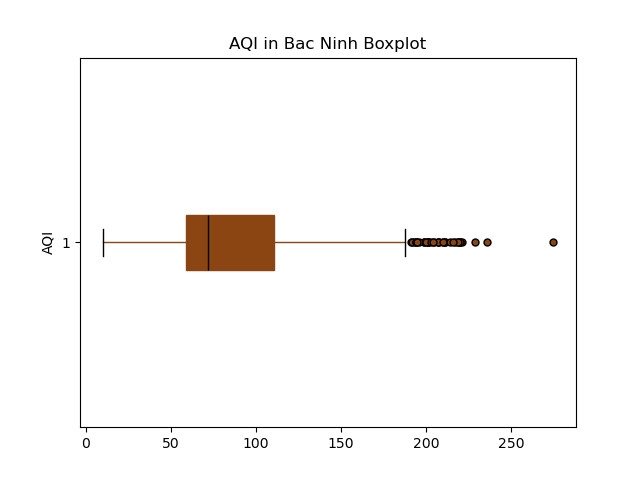
\includegraphics[width=1\textwidth]{bibliography/figure/bn_box.jpg}
        \caption{BacNinh AQI's boxplot}
        \label{fig:1}
    \end{minipage}
    \hfill
    \begin{minipage}{0.23\textwidth}
        \centering
        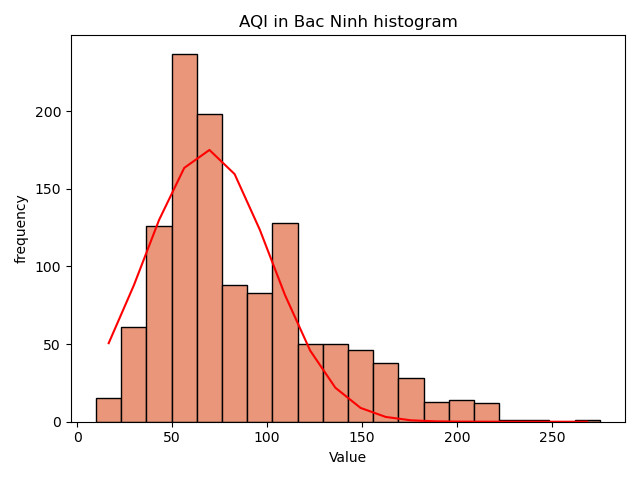
\includegraphics[width=1\textwidth]{bibliography/figure/bn_his.jpg}
        \caption{BacNinh AQI's hostogram}
        \label{fig:2}
    \end{minipage}
\end{figure}

\begin{figure}[H]
    \centering
    \begin{minipage}{0.23\textwidth}
        \centering
        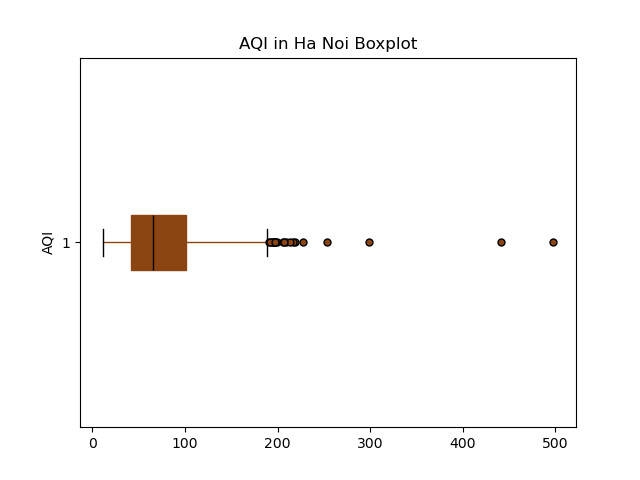
\includegraphics[width=1\textwidth]{bibliography/figure/hn_box.jpg}
        \caption{HaNoi AQI's boxplot}
        \label{fig:1}
    \end{minipage}
    \hfill
    \begin{minipage}{0.23\textwidth}
        \centering
        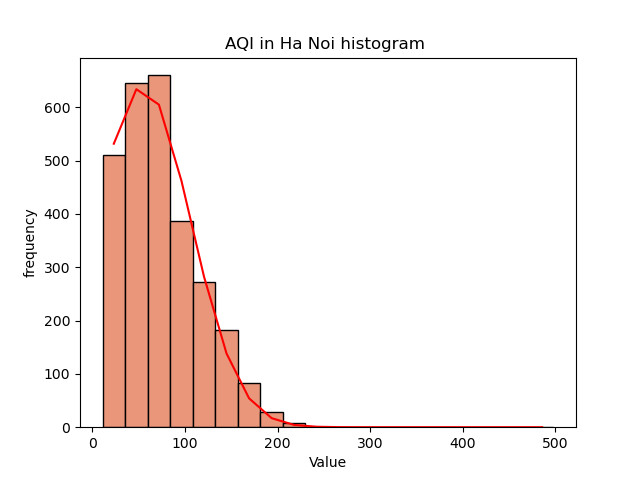
\includegraphics[width=1\textwidth]{bibliography/figure/hn_his.jpg}
        \caption{HaNoi AQI's hostogram}
        \label{fig:2}
    \end{minipage}
\end{figure}

\begin{figure}[H]
    \centering
    \begin{minipage}{0.23\textwidth}
        \centering
        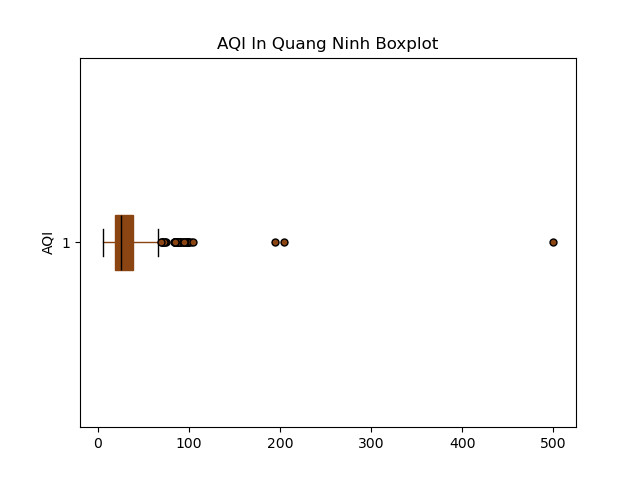
\includegraphics[width=1\textwidth]{bibliography/figure/qn_box.jpg}
        \caption{QuangNinh AQI's boxplot}
        \label{fig:1}
    \end{minipage}
    \hfill
    \begin{minipage}{0.23\textwidth}
        \centering
        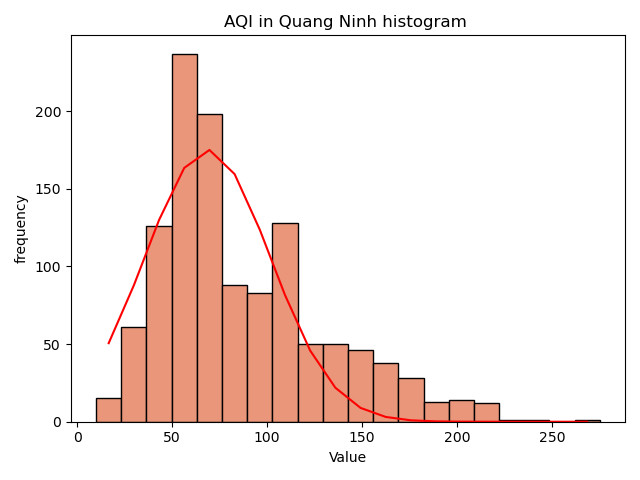
\includegraphics[width=1\textwidth]{bibliography/figure/qn_his.jpg}
        \caption{QuangNinh AQI's hostogram}
        \label{fig:2}
    \end{minipage}
\end{figure}

\section{Phương pháp luận}
\subsection{Gauss newton method nonlinear}
\subsubsection{Least Squares}
Khoảng cách giữa một đường cong được khớp và một quan sát được gọi là sai số dư, hoặc lỗi.

\begin{center}
    $Residuals = y_i - \widehat{y}_i$
\end{center}

Tổng của các sai số bình phương được tính bằng phương trình sau:

\begin{center}
    $SSE = \sum_{i=1}^{n}(y_i - \widehat{y}_i)^2$
\end{center}

Trong đó: \\
\indent\textbullet\ \(y_i\) là các giá trị quan sát được\\
\indent\textbullet\ \(\widehat{y}_i\) là các giá trị khớp\\

\subsubsection{Phương pháp Newton}
Với hàm \( y = y_0 e^{-kt} \), chúng ta tìm giá trị nhỏ nhất của SSE. Chúng ta tìm giá trị \(k\) bằng phương pháp Newton.

\begin{center}
    $SSE = \sum_{i}^{n}(y_i - y_0 e^{-kt_i})^2$
\end{center}

\begin{center}
    \(k_{\text{new}} = k_{\text{old}} - \frac{f'(k_{\text{old}})}{f''(k_{\text{old}})}\)
\end{center}

Hoặc chúng ta có thể giải thích bằng ma trận Hessian như sau:

\begin{center}
    \[
        \begin{pmatrix}
            k_{\text{new}} \\ y_{0,\text{new}}
        \end{pmatrix} =
        \begin{pmatrix}
            k_{\text{old}} \\ y_{0,\text{old}}
        \end{pmatrix} - H^{-1}G
    \]
\end{center}

Trong đó: \\
\indent\textbullet\ \(H = \begin{bmatrix}
    \frac{\partial^2 f}{\partial k^2}            & \frac{\partial^2 f}{\partial k \partial y_0} \\
    \frac{\partial^2 f}{\partial y_0 \partial k} & \frac{\partial^2 f}{\partial y_0^2}
\end{bmatrix}\)\\
\indent\textbullet\ \(G = \begin{bmatrix}
    \frac{\partial f}{\partial k} \\ \frac{\partial f}{\partial y_0}
\end{bmatrix}\)\\

Vấn đề với phương pháp Newton trong hồi quy phi tuyến là việc tính toán ma trận Hessian và nghịch đảo của nó gặp khó khăn. Để giải quyết vấn đề này, phương pháp Gauss-Newton thay thế bằng cách xấp xỉ ma trận Hessian.

Chúng ta có thể viết lại SSE như sau:
\begin{center}
    $SSE = \sum_{i}^{n}r_i^2 = r^T r$
\end{center}

Trong đó: \\
\indent\textbullet\ \(r\) là một vector chứa các sai số dư \\

\subsubsection{Phương pháp Gauss-Newton}
Chúng ta lấy đạo hàm của SSE theo các tham số trong mô hình bằng quy tắc chuỗi, chúng ta có được phương trình sau:
\begin{center}
    \(
    \frac{\partial SSE}{\partial \beta_j} = 2\sum_{i}^{n} r_i \frac{\partial r_i}{\partial \beta_j}
    \)
\end{center}

Sau đó, bỏ số hai vì nó sẽ không ảnh hưởng đến việc ước tính các tham số. Tương ứng với ma trận Jacobian.

\begin{center}
    \(
    J_r = \begin{bmatrix}
        \frac{\partial r_1}{\partial \beta_1} & \frac{\partial r_1}{\partial \beta_2} \\
        \frac{\partial r_2}{\partial \beta_1} & \frac{\partial r_2}{\partial \beta_2} \\
        \vdots                                & \vdots                                \\
        \frac{\partial r_n}{\partial \beta_1} & \frac{\partial r_n}{\partial \beta_2}
    \end{bmatrix}
    \)
\end{center}

Với phương trình sau cho tổng các sai số bình phương (SSE):
\[
    SSE = \sum_{i=1}^{n} (y_i - y_0 e^{-kt_i})^2
\]
Chúng ta có:
\begin{center}
    \(
    \frac{\partial^2 {SSE}}{\partial \beta_j \partial \beta_k} = \sum_{i}^{n} \left( \frac{\partial r_i}{\partial \beta_j} \frac{\partial r_i}{\partial \beta_k} + r_i \frac{\partial^2 r_i}{\partial \beta_j \partial \beta_k} \right)
    \)
\end{center}

Sự khác biệt chính giữa phương pháp Newton và Gauss-Newton là phương pháp Gauss-Newton bỏ qua \(r_i \frac{\partial^2 r_i}{\partial \beta_j \partial \beta_k}\).
Do đó, đạo hàm bậc hai được xấp xỉ bằng hàm sau:
\begin{center}
    \(
    \frac{\partial^2 {SSE}}{\partial \beta_j \partial \beta_k} \approx \sum_{i}^{n} \left( \frac{\partial r_i}{\partial \beta_j} \frac{\partial r_i}{\partial \beta_k} \right) = J^T_r J_r
    \)
\end{center}

Sử dụng quy tắc cập nhật sau trong phương pháp Newton. Đối với Gauss-Newton, đơn giản chỉ cần cắm vào xấp xỉ cho ma trận Hessian và gradient.

\begin{center}
    \[
        \begin{pmatrix}
            k_{\text{new}} \\ y_{0,\text{new}}
        \end{pmatrix} =
        \begin{pmatrix}
            k_{\text{old}} \\ y_{0,\text{old}}
        \end{pmatrix} - (J^T_r J_r)^{-1} J^T_r r
    \]
\end{center}

Với \(\beta\) là một vector cột với các tham số được ước tính. Đối với ví dụ đơn giản chỉ ước tính hai tham số, phương trình trông như sau:

\begin{center}
    \[
        \beta_{\text{new}} = \beta_{\text{old}} - (J^T_r J_r)^{-1} J^T_r r(\beta_{\text{old}})
    \]
    \[
        \begin{pmatrix}
            k_{\text{new}} \\ y_{0,\text{new}}
        \end{pmatrix} =
        \begin{pmatrix}
            k_{\text{old}} \\ y_{0,\text{old}}
        \end{pmatrix} - (J^T_r J_r)^{-1} J^T_r r \begin{pmatrix}
            k_{\text{old}} \\ y_{0,\text{old}}
        \end{pmatrix}
    \]
\end{center}

\subsection{Gated Recurrent Unit (GRU)}
\subsubsection{Đơn vị tuần hoàn trong mạng nơ-ron}
Trước khi chúng ta đi vào chi tiết về GRU, hãy xem xét một đơn vị tuần hoàn thông thường trong mạng nơ-ron. Đơn vị này được sử dụng để xử lý dữ liệu tuần tự, chẳng hạn như chuỗi văn bản, âm thanh hoặc dữ liệu thời gian.

Mỗi đơn vị tuần hoàn có một trạng thái ẩn (hidden state) và nhận đầu vào từ bước thời gian trước đó. Nó sử dụng thông tin từ trạng thái ẩn và đầu vào hiện tại để tính toán trạng thái ẩn mới.

\subsubsection{GRU là gì?}
GRU là một biến thể của đơn vị tuần hoàn, được thiết kế để giải quyết một số vấn đề của kiến trúc LSTM (Long Short-Term Memory).

Sự khác biệt chính giữa GRU và LSTM nằm ở cách xử lý trạng thái ẩn và ô nhớ:

\begin{itemize}
    \item \textbf{LSTM}: Sử dụng ba cổng (input gate, output gate và forget gate) để duy trì trạng thái của ô nhớ riêng biệt.
    \item \textbf{GRU}: Không có ô nhớ riêng biệt, thay vào đó, nó sử dụng một “vector kích hoạt ứng viên” và hai cổng (reset gate và update gate).
\end{itemize}

\begin{itemize}
    \item \textbf{Cổng đặt lại (reset gate)}: Quyết định bao nhiêu trạng thái ẩn trước đó cần quên.
    \item \textbf{Cổng cập nhật (update gate)}: Quyết định bao nhiêu của vector kích hoạt ứng viên cần tích hợp vào trạng thái ẩn mới.
\end{itemize}

\subsubsection{Cổng xóa và cổng cập nhật}
Đầu tiên ta giới thiệu cổng xóa và cổng cập nhật. Ta thiết kế chúng thành các vector có các phần tử trong khoảng  (0,1)
để có thể biểu diễn các tổ hợp lồi. Chẳng hạn, một biến xóa cho phép kiểm soát bao nhiêu phần của trạng thái trước đây được giữ lại. Tương tự, một biến cập nhật cho phép kiểm soát bao nhiêu phần của trạng thái mới sẽ giống trạng thái cũ.


\begin{figure}[H]
    \centering
    \begin{minipage}{0.23\textwidth}
        \centering
        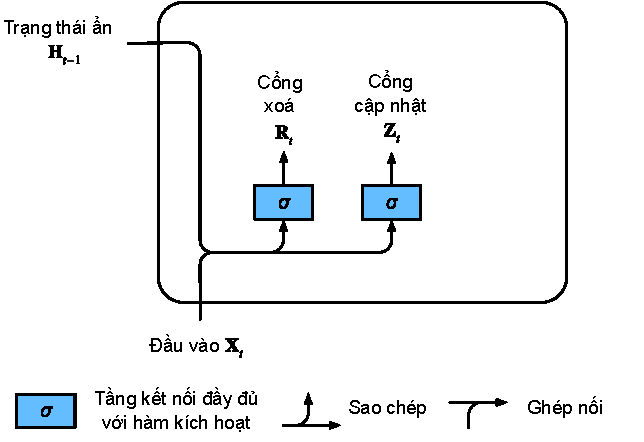
\includegraphics[width=1\textwidth]{bibliography/figure/GRU/gru_1.pdf}
        \caption{Cổng xóa và cổng cập nhật trong GRU}
        \label{fig:gru_del_up}
    \end{minipage}

\end{figure}

Ta bắt đầu bằng việc thiết kế các cổng tạo ra các biến này. Hình \ref{fig:gru_del_up}
minh họa các đầu vào cho cả cổng xóa và cổng cập nhật trong GRU, với đầu vào ở bước thời gian hiện tại  \(\mathbf{X}_t \)
và trạng thái ẩn ở bước thời gian trước đó  \(\mathbf{H}_{t-1} \). Đầu ra được tạo bởi một tầng kết nối đầy đủ với hàm kích hoạt sigmoid.

Tại bước thời gian $t$, với đầu vào minibatch là $\mathbf{X}_t \in \mathbb{R}^{n \times d}$ (số lượng mẫu: $n$, số lượng đầu vào: $d$) và trạng thái ẩn ở bước thời gian gần nhất là $\mathbf{H}_{t-1} \in \mathbb{R}^{n \times h}$ (số lượng trạng thái ẩn: $h$), cổng xóa $\mathbf{R}_t \in \mathbb{R}^{n \times h}$ và cổng cập nhật $\mathbf{Z}_t \in \mathbb{R}^{n \times h}$ được tính như sau:

\begin{equation*}
    \mathbf{R}_t = \sigma(\mathbf{X}_t \mathbf{W}_{xr} + \mathbf{H}_{t-1} \mathbf{W}_{hr} + \mathbf{b}_r)
\end{equation*}
\begin{equation*}
    \mathbf{Z}_t = \sigma(\mathbf{X}_t \mathbf{W}_{xz} + \mathbf{H}_{t-1} \mathbf{W}_{hz} + \mathbf{b}_z).
\end{equation*}

Ở đây, $\mathbf{W}_{xr}, \mathbf{W}_{xz} \in \mathbb{R}^{d \times h}$ và $\mathbf{W}_{hr}, \mathbf{W}_{hz} \in \mathbb{R}^{h \times h}$ là các tham số trọng số và $\mathbf{b}_r, \mathbf{b}_z \in \mathbb{R}^{1 \times h}$ là các hệ số điều chỉnh. Ta sẽ sử dụng hàm sigmoid để biến đổi các giá trị đầu vào nằm trong khoảng $(0, 1)$.

\subsubsection{Hoạt động của cổng xóa}
Trong RNN thông thường, ta cập nhật trọng thái cổng xóa theo công thức
\[
    \mathbf{H}_t = \tanh(\mathbf{X}_t \mathbf{W}_{xh} + \mathbf{H}_{t-1} \mathbf{W}_{hh} + \mathbf{b}_h).
\]

Hình \ref{fig:gru_del} minh họa luồng tính toán sau khi áp dụng cổng xóa. Ký hiệu \(\bigodot\) biểu thị phép nhân theo từng phần tử giữa các tensor.

\begin{figure}[H]
    \centering
    \begin{minipage}{0.23\textwidth}
        \centering
        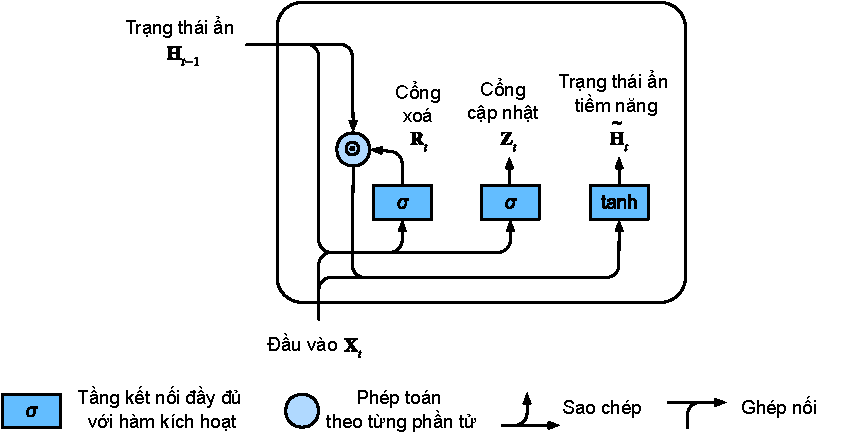
\includegraphics[width=1\textwidth]{bibliography/figure/GRU/gru_2.pdf}
        \caption{Tính toán trạng thái tiềm năng trong một GRU. Phép nhân được thực hiện theo phần tử}
        \label{fig:gru_del}
    \end{minipage}

\end{figure}

\begin{thebibliography}{00}
    \bibitem{b1}  P. T. Huong, "Linear regression, polynomial regression, and applications,
    master’s thesis in science," 2015.
\end{thebibliography}

\end{document}
